\documentclass[14pt,a4paper]{extarticle}
\usepackage{fontspec}
\setmainfont{Times New Roman}
\usepackage[english,russian]{babel}
\usepackage{graphicx} % Required for inserting images
\usepackage[top=20mm,bottom=20mm,left=30mm,right=15mm]{geometry}
\usepackage{xcolor}
\usepackage{setspace}
\usepackage{tabularx}
\usepackage{fancyhdr}
\usepackage{caption}
\usepackage{graphicx}
\usepackage{placeins}
\usepackage{caption}
\usepackage{subcaption}
\usepackage{amsmath}
\usepackage{float}

\setlength{\parindent}{15mm}
\setstretch{1.5}
\linespread{1.25}
\tolerance=1
\emergencystretch=\maxdimen
\hyphenpenalty=10000
\exhyphenpenalty=10000
\usepackage{titlesec}
\titleformat{\section}[hang]{\normalfont\bfseries}{\thesection}{}{}
\titlespacing{\section}{15mm}{0pt}{0pt}
\captionsetup[figure]{name = {Рисунок}, labelsep = endash}

\begin{document}
\begin{titlepage}
    \begin{center}
    {\bfseries
    МИНОБРНАУКИ РОССИИ \\ САНКТ-ПЕТЕРБУРГСКИЙ ГОСУДАРСТВЕННЫЙ \\ ЭЛЕКТРОТЕХНИЧЕСКИЙ УНИВЕРСИТЕТ \\ <<ЛЭТИ>> ИМ. В.И. УЛЬЯНОВА (ЛЕНИНА)\\Кафедра САПР \vspace{0.23\textheight}
    
    ОТЧЕТ \\ по практической работе №8 \\ по дисциплине <<Информационные технологии>> \\ Тема: Линейная регрессия и системы линейных уравнений. \\
    \vspace{0.28\textheight}
        }
        \begin{table}[h!]
            \begin{tabularx}{\textwidth}{p{60mm}X>{\centering\arraybackslash}p{45mm}}
                Студент гр. 4352 & \_\_\_\_\_\_\_\_\_\_\_\_\_\_\_\_\_\_\_\_ & {Колесникова М. А.} \\ [5.4mm]  
                Преподаватель    & \_\_\_\_\_\_\_\_\_\_\_\_\_\_\_\_\_\_\_\_ & {Копец Е. Е.} \\ [5.4mm]
            \end{tabularx}
        \end{table}
    Санкт-Петербург\par
        2025
    \end{center}
\end{titlepage}
\setcounter{page}{2}

\section*{Цель работы.}

Научиться решать вручную и с помощью sympy системы линейных алгебраических уравнений.
А также с помощью переопределённых СЛАУ находить среднее крадратичное значение. 

\section*{Основные теоретические положения.}

В первом задании нужно решить систему линейных уравнений вручную.
Сделаем это приводя матрицы к ступенчатому виду.

1.
\[
\left\{
\begin{array}{l}
2x + 5y = 11 \\
7x - 3y = -23
\end{array}
\right.
\]

Решение:\\
\[
\left(\begin{array}{cc|c}
2 & 5 & 11 \\
7 & -3 & -23
\end{array}\right)
\sim
\left(\begin{array}{cc|c}
2 & 5 & 11 \\
0 & -\frac{41}{2} & -\frac{123}{2}
\end{array}\right)
;\]
\[
-\frac{41}{2}y = -\frac{123}{2} \Rightarrow y = 3
;\]
\[
2x + 5 \cdot 3 = 11 \Rightarrow x = -2
.\]

Ответ: \( x = -2 \), \( y = 3 \).

Матричное уравнение:\\
\[\begin{pmatrix}2 & 5 \\7 & -3\end{pmatrix}\begin{pmatrix}x \\y\end{pmatrix}=\begin{pmatrix}11 \\-23\end{pmatrix}.\]

2.
\[
\left\{
\begin{array}{l}
-3x + y = -2 \\
3x + 5y = 8
\end{array}
\right.
\]

Решение:\\
\[
\left(\begin{array}{cc|c}
-3 & 1 & -2 \\
3 & 5 & 8
\end{array}\right)
\sim
\left(\begin{array}{cc|c}
-3 & 1 & -2 \\
0 & 6 & 6
\end{array}\right)
;\]
\[
6y = 6 \Rightarrow y = 1
;\]
\[
-3x + 1 = -2 \Rightarrow x = 1
.\]

Ответ: \( x = 1 \), \( y = 1 \).

Матричное уравнение:
\[\begin{pmatrix}-3 & 1 \\3 & 5\end{pmatrix}\begin{pmatrix}x \\y\end{pmatrix}=\begin{pmatrix}-2 \\8\end{pmatrix}.\]

3.
\[
\left\{
\begin{array}{l}
2x + 3y = 12 \\
3x - y = 7
\end{array}
\right.
\]

Решение:
\[
\left(\begin{array}{cc|c}
2 & 3 & 12 \\
3 & -1 & 7
\end{array}\right)
\sim
\left(\begin{array}{cc|c}
2 & 3 & 12 \\
0 & -\frac{11}{2} & -11
\end{array}\right)
;\]
\[
-\frac{11}{2}y = -11 \Rightarrow y = 2
;\]
\[
2x + 3 \cdot 2 = 12 \Rightarrow x = 3
.\]

Ответ: \( x = 3 \), \( y = 2 \).

Матричное уравнение:
\[\begin{pmatrix}2 & 3 \\3 & -1\end{pmatrix}\begin{pmatrix}x \\y\end{pmatrix}=\begin{pmatrix}12 \\7\end{pmatrix}.\]

4.
\[
\left\{
\begin{array}{l}
x + y + 2z = -1 \\
2x - y + 2z = -4 \\
4x + y + 4z = -2
\end{array}
\right.
\]

Решение:\\
\[
\left(\begin{array}{ccc|c}
1 & 1 & 2 & -1 \\
2 & -1 & 2 & -4 \\
4 & 1 & 4 & -2
\end{array}\right)
\sim
\left(\begin{array}{ccc|c}
1 & 1 & 2 & -1 \\
0 & -3 & -2 & -2 \\
0 & -3 & -4 & 2
\end{array}\right)
\sim
\left(\begin{array}{ccc|c}
1 & 1 & 2 & -1 \\
0 & -3 & -2 & -2 \\
0 & 0 & -2 & 4
\end{array}\right)
;\]
\[
-2z = 4 \Rightarrow z = -2
;\]
\[
-3y - 2(-2) = -2 \Rightarrow y = 2
;\]
\[
x + 2 + 2(-2) = -1 \Rightarrow x = 1
.\]

Ответ: \( x = 1 \), \( y = 2 \), \( z = -2 \).

Матричное уравнение:
\[\begin{pmatrix}1 & 1 & 2 \\2 & -1 & 2 \\4 & 1 & 4\end{pmatrix}\begin{pmatrix}x \\y \\z\end{pmatrix}=\begin{pmatrix}-1 \\-4 \\-2\end{pmatrix}.\]

Умножение матриц на векторы:

1.
\[
\begin{pmatrix} 2 & 5 \\ 7 & -3\end{pmatrix}
\begin{pmatrix} 2 \\ 3\end{pmatrix} = \begin{pmatrix} 19 \\ 5\end{pmatrix}
;\]

2.
\[
\begin{pmatrix} -3 & 1 \\ 3 & 5\end{pmatrix}
\begin{pmatrix} 1 \\ 3\end{pmatrix} = \begin{pmatrix} 0 \\ 18 \end{pmatrix}
;\]

3.
\[
\begin{pmatrix} 2 & 3 \\ 3 & -1\end{pmatrix}
\begin{pmatrix} 4 \\ 2\end{pmatrix} = \begin{pmatrix} 14 \\ 10 \end{pmatrix}
;\]

4.
\[
\begin{pmatrix} 1 & 1 & 2 \\ 2 & -1 & 2 \\4 & 1 & 4\end{pmatrix}
\begin{pmatrix} 2 \\ 3 \\ 5\end{pmatrix} = \begin{pmatrix} 15 \\ 11 \\ 31 \end{pmatrix}
.\]

В третьем задании нужно решить системы линейных уравнений:

1.
\[
\begin{cases} 
-x + 7y = -34 \\ 
8x + 8y = -48 
\end{cases}
\]

Решение:
\[
\left(\begin{array}{cc|c}
-1 & 7 & -34 \\
8 & 8 & -48
\end{array}\right)
\sim
\left(\begin{array}{cc|c}
-1 & 7 & -34 \\
0 & 64 & -320
\end{array}\right)
;\]
\begin{align*}
    64y &= -320 \Rightarrow y = -5; \\
    -x + 7(-5) &= -34 \Rightarrow x = -1.
    \end{align*}

Ответ: \( x = -1 \), \( y = -5 \).

2.
\[
\begin{cases} 
4x - 7y = -4 \\ 
3x - 4y = -3 
\end{cases}
\]

Решение:
\[
\left(\begin{array}{cc|c}
4 & -7 & -4 \\
3 & -4 & -3
\end{array}\right)
\sim
\left(\begin{array}{cc|c}
4 & -7 & -4 \\
0 & \frac{5}{4} & 0
\end{array}\right)
;\]
\begin{align*}
    \frac{5}{4}y &= 0 \Rightarrow y = 0; \\
    4x - 7(0) &= -4 \Rightarrow x = -1.
    \end{align*}

Ответ: \( x = -1 \), \( y = 0 \).

3.
\[
\begin{cases} 
8a - 4b = 64 \\ 
-3a + 3b = -21 
\end{cases}
\]

Решение:
\[
\left(\begin{array}{cc|c}
8 & -4 & 64 \\
-3 & 3 & -21
\end{array}\right)
\sim
\left(\begin{array}{cc|c}
8 & -4 & 64 \\
0 & \frac{3}{2} & 3
\end{array}\right)
;\]
\begin{align*}
    \frac{3}{2}b &= 3 \Rightarrow b = 2; \\
    8a - 4(2) &= 64 \Rightarrow a = 9.
    \end{align*}

Ответ: \( a = 9 \), \( b = 2 \).

4.
\[
\begin{cases} 
5x_1 + 7x_2 - 5x_3 = -47 \\ 
-2x_2 + 2x_3 = 10 \\ 
-4x_1 - 8x_2 - 7x_3 = 63 
\end{cases}
\]

Решение:
\[
\left(\begin{array}{ccc|c}
5 & 7 & -5 & -47 \\
0 & -2 & 2 & 10 \\
-4 & -8 & -7 & 63
\end{array}\right)
\sim
\left(\begin{array}{ccc|c}
5 & 7 & -5 & -47 \\
0 & -2 & 2 & 10 \\
0 & -\frac{12}{5} & -11 & \frac{107}{5}
\end{array}\right)
\sim\]
\[
\sim
\left(\begin{array}{ccc|c}
5 & 7 & -5 & -47 \\
0 & -2 & 2 & 10 \\
0 & 0 & -\frac{67}{5} & \frac{67}{5}
\end{array}\right)
;\]
\begin{align*}
    -\frac{67}{5}x_3 &= \frac{67}{5} \Rightarrow x_3 = -1; \\
    -2x_2 + 2(-1) &= 10 \Rightarrow x_2 = -6; \\
    5x_1 + 7(-6) - 5(-1) &= -47 \Rightarrow x_1 = -2.
    \end{align*}

Ответ: \( x_1 = -2 \), \( x_2 = -6 \), \( x_3 = -1 \).

Результаты программы совпали с полученными значениями (рис. \ref{pic:sly1}).
\begin{figure}[h!]
    \centering
    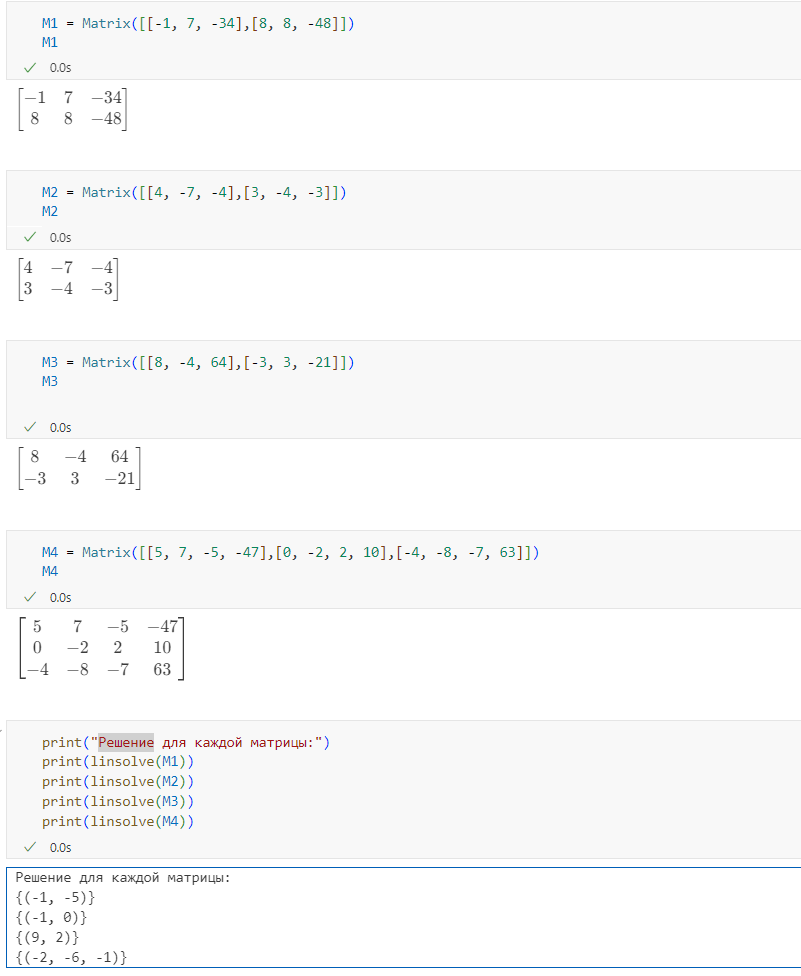
\includegraphics[scale=0.6]{pic8/1.png}
    \caption{Проверка решений СЛАУ}
    \label{pic:sly1}
\end{figure}
\FloatBarrier

В четвёртом задании нужно умножить матрицы на вектора:

1.\[\begin{pmatrix} -1 & 7 \\ 8 & 8 \end{pmatrix}\begin{pmatrix} -1 \\ -5 \end{pmatrix} 
= \begin{pmatrix} (-1) \cdot (-1) + 7 \cdot (-5) \\ 8 \cdot (-1) + 8 \cdot (-5) \end{pmatrix}=
\begin{pmatrix} 1 - 35 \\ -8 - 40 \end{pmatrix}
=\begin{pmatrix} -34 \\ -48 \end{pmatrix};\]

2. \[\begin{pmatrix} 4 & -7 \\ 3 & -4 \end{pmatrix}\begin{pmatrix} -1 \\ 0 \end{pmatrix} 
= \begin{pmatrix} 4 \cdot (-1) + (-7) \cdot 0 \\ 3 \cdot (-1) + (-4) \cdot 0 \end{pmatrix}
=\begin{pmatrix} -4 + 0 \\ -3 + 0 \end{pmatrix}
=\begin{pmatrix} -4 \\ -3 \end{pmatrix};\]

3. \[\begin{pmatrix} 8 & -4 \\ -3 & 3 \end{pmatrix}\begin{pmatrix} 9 \\ 2 \end{pmatrix} 
= \begin{pmatrix} 8 \cdot 9 + (-4) \cdot 2 \\ -3 \cdot 9 + 3 \cdot 2 \end{pmatrix}
=\begin{pmatrix} 72 - 8 \\ -27 + 6 \end{pmatrix}
=\begin{pmatrix} 64 \\ -21 \end{pmatrix};\]

4. \[\begin{pmatrix} 5 & 7 & -5 \\ 0 & -2 & 2 \\ -4 & -8 & -7 \end{pmatrix}\begin{pmatrix} -2 \\ -6 \\ -1\end{pmatrix}
=\begin{pmatrix} -47 \\ 10 \\ 63 \end{pmatrix}.\]

Результаты программы совпадают с найденными значениями (рис. \ref{pic:12}, \ref{pic:34}).
\begin{figure}[h!]
    \centering
    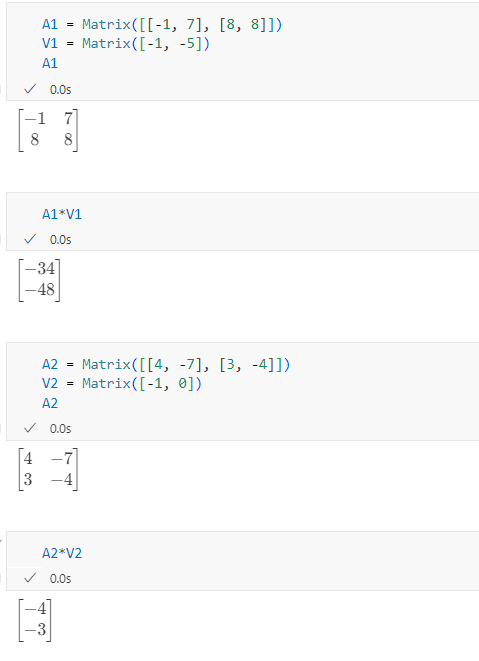
\includegraphics[scale=0.7]{pic8/2.1.png}
    \caption{Проверка 1 и 2}
    \label{pic:12}
\end{figure}
\FloatBarrier
\begin{figure}[h!]
    \centering
    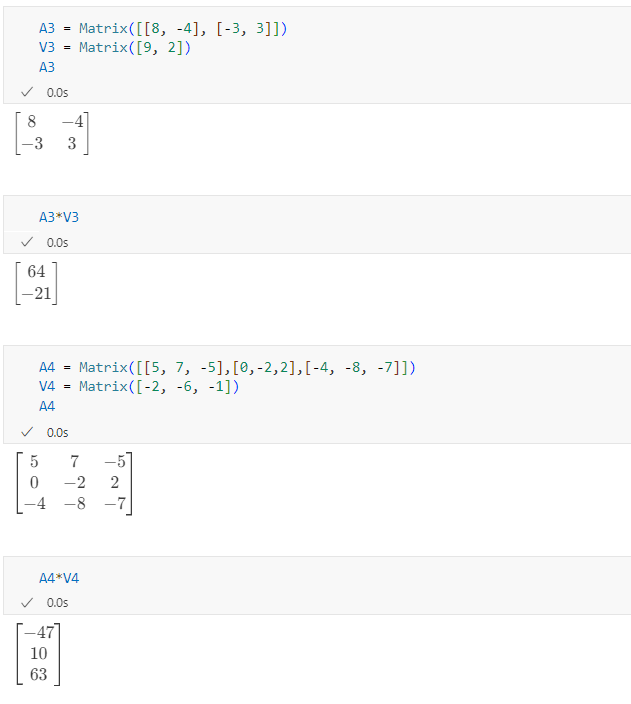
\includegraphics[scale=0.6]{pic8/2.2.png}
    \caption{Проверка 3 и 4}
    \label{pic:34}
\end{figure}
\FloatBarrier

В пятом задании нужно решить переопределённую СЛАУ.\\

Дана система уравнений:
\[
\begin{cases}
5x + 7y - 5z = -47 \\
-2y + 2z = 10 \\
-4x - 8y - 7z = 63
\end{cases}
\]

Запишем расширенную матрицу системы:
\[
\left(\begin{array}{ccc|c}
5 & 7 & -5 & -47 \\
0 & -2 & 2 & 10 \\
-4 & -8 & -7 & 63
\end{array}\right)
.\]

Обнулим элемент $a_{31}$ ($-4$) с помощью строки $R_1$:
\[
R_3 \rightarrow R_3 + \frac{4}{5}R_1
:\]
\[
\left(\begin{array}{ccc|c}
5 & 7 & -5 & -47 \\
0 & -2 & 2 & 10 \\
0 & -\frac{12}{5} & -11 & \frac{127}{5}
\end{array}\right)
.\]

Обнулим элемент $a_{32}$ ($-\frac{12}{5}$) с помощью строки $R_2$:
\[
R_3 \rightarrow R_3 - \frac{6}{5}R_2
:\]
\[
\left(\begin{array}{ccc|c}
5 & 7 & -5 & -47 \\
0 & -2 & 2 & 10 \\
0 & 0 & -\frac{67}{5} & \frac{67}{5}
\end{array}\right)
.\]

Найдем $z$ из третьей строки:
\[
-\frac{67}{5}z = \frac{67}{5} \Rightarrow z = -1
:\]

Найдем $y$ из второй строки:
\[
-2y + 2(-1) = 10 \Rightarrow y = -6.
\]

Найдем $x$ из первой строки:
\[
5x + 7(-6) - 5(-1) = -47 \Rightarrow x = -2.
\]

Ответ:
\[{
\begin{pmatrix}
x \\
y \\
z
\end{pmatrix}
=
\begin{pmatrix}
-2 \\
-6 \\
-1
\end{pmatrix}
}
.\]

Для нахождения MSE пишем код используя numpy (рис. \ref{pic:mse}).

\begin{figure}[h!]
    \centering
    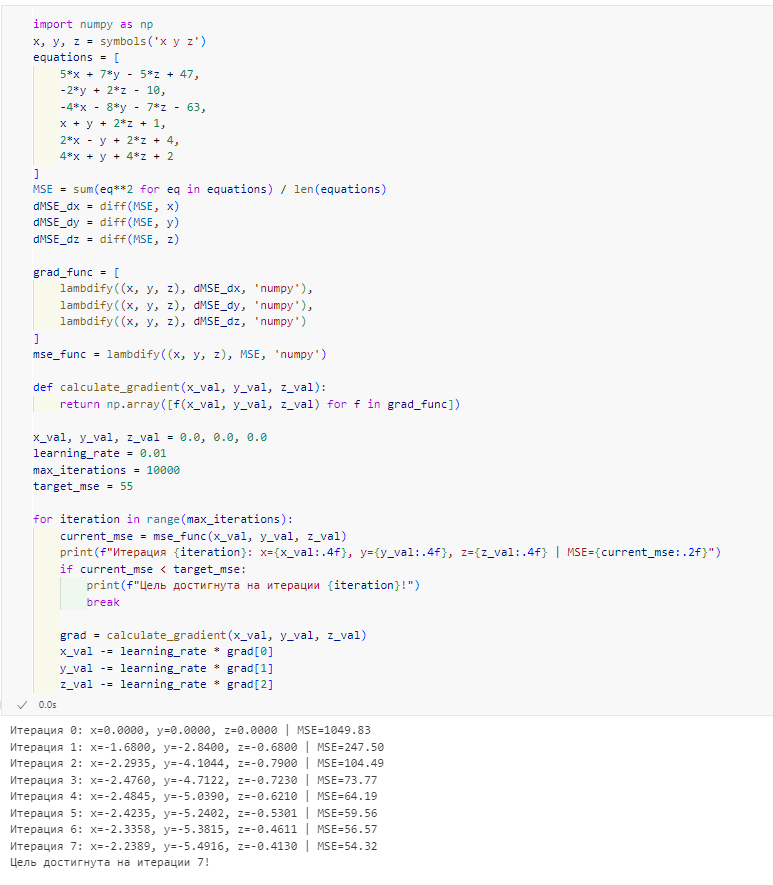
\includegraphics[scale=0.7]{pic8/3.png}
    \caption{Нахождение MSE меньше 55}
    \label{pic:mse}
\end{figure}
\FloatBarrier
\section*{Вывод.}

В ходе работы было изучено решение систем алгебраических уравнений, умножение матрицы на вектор.
А также было найдено среднее квадратичное отклонение для переопределённой СЛАУ.

\end{document}